%% Poster template with TikZ figures.
\documentclass[36pt]{sciposter}
\usepackage{preposterTikz} % package with poster preamble.
\geometry{paperwidth=90cm,paperheight=100cm,centering,
    textwidth=85cm,textheight=94cm,left=0cm,top=2cm}
\pgfplotsset{compat=1.18}
%********************************************************************
%********************************************************************
\begin{document}

\onehalfspacing

%% Fill in the commands below with your project data.
\newcommand{\posterTitle}{Topographic Controls on Alpine Snow Depth:} % main poster title
\newcommand{\posterSubtitle}{Multi-Temporal UAV Data Analysis Using Machine Learning } % Use only if a second line is needed.
% If no subtitle is needed, keep the braces empty: {}.
\newcommand{\authorNames}{Andersch$^{(a)}$, Elias, Wundram$^{(a)}$, Kjell} % author names
\newcommand{\institutionName}{$(a)$ Applied Earth Observation, University of Würzburg} % affiliation

% Backward-compatible aliases.
\let\tituloposter\posterTitle
\let\titulogrande\posterSubtitle
\let\nome\authorNames
\let\instituicao\institutionName

%% Header built with TikZ.
\posterHeader{Figures/Logos/eagle_master_full_noText_bw_white-e1463595440895.png}{Figures/Logos/uni-wuerzburg-logo.png}{BoxCol}
\vspace{5cm} % spacing
\section*{\tituloA{SUMMARY}}


Lorem ipsum dolor sit amet, consectetur adipiscing elit. Aliquam porta justo vel vehicula cursus. Quisque porta lectus sit amet mattis accumsan. Donec nulla leo, vestibulum quis suscipit eu, porta vel tellus. Phasellus sed pellentesque mauris. Mauris posuere massa magna, at gravida nibh dapibus nec. Curabitur non nibh non tortor elementum hendrerit id id risus. 
%% Text in two columns.
\begin{multicols}{2}
%% Paragraph formatting.
\setlength{\parindent}{3em}
\section*{\tituloA{OBJECTIVES}}

\noindent
The aim of this project was to predict snow accumulation and depth using indices. This approach was chosen to bypass the time-consuming processing of DEMs and provide an efficient prediction method.
\section*{\tituloA{METHODOLOGY}}

%\begin{enumerate}
%	\begin{equation}
%		DSM_{snow depth} = DSM_{winter} - DSM_{summer}
%	\end{equation}
%	\item Calculate indices with whitebox tools
%	\item Create chunks of the study area
%	\item Train and optimize a HistGradientBoostingRegressor
%s\end{enumerate}
\begin{figure}[h]
	\begin{center}
		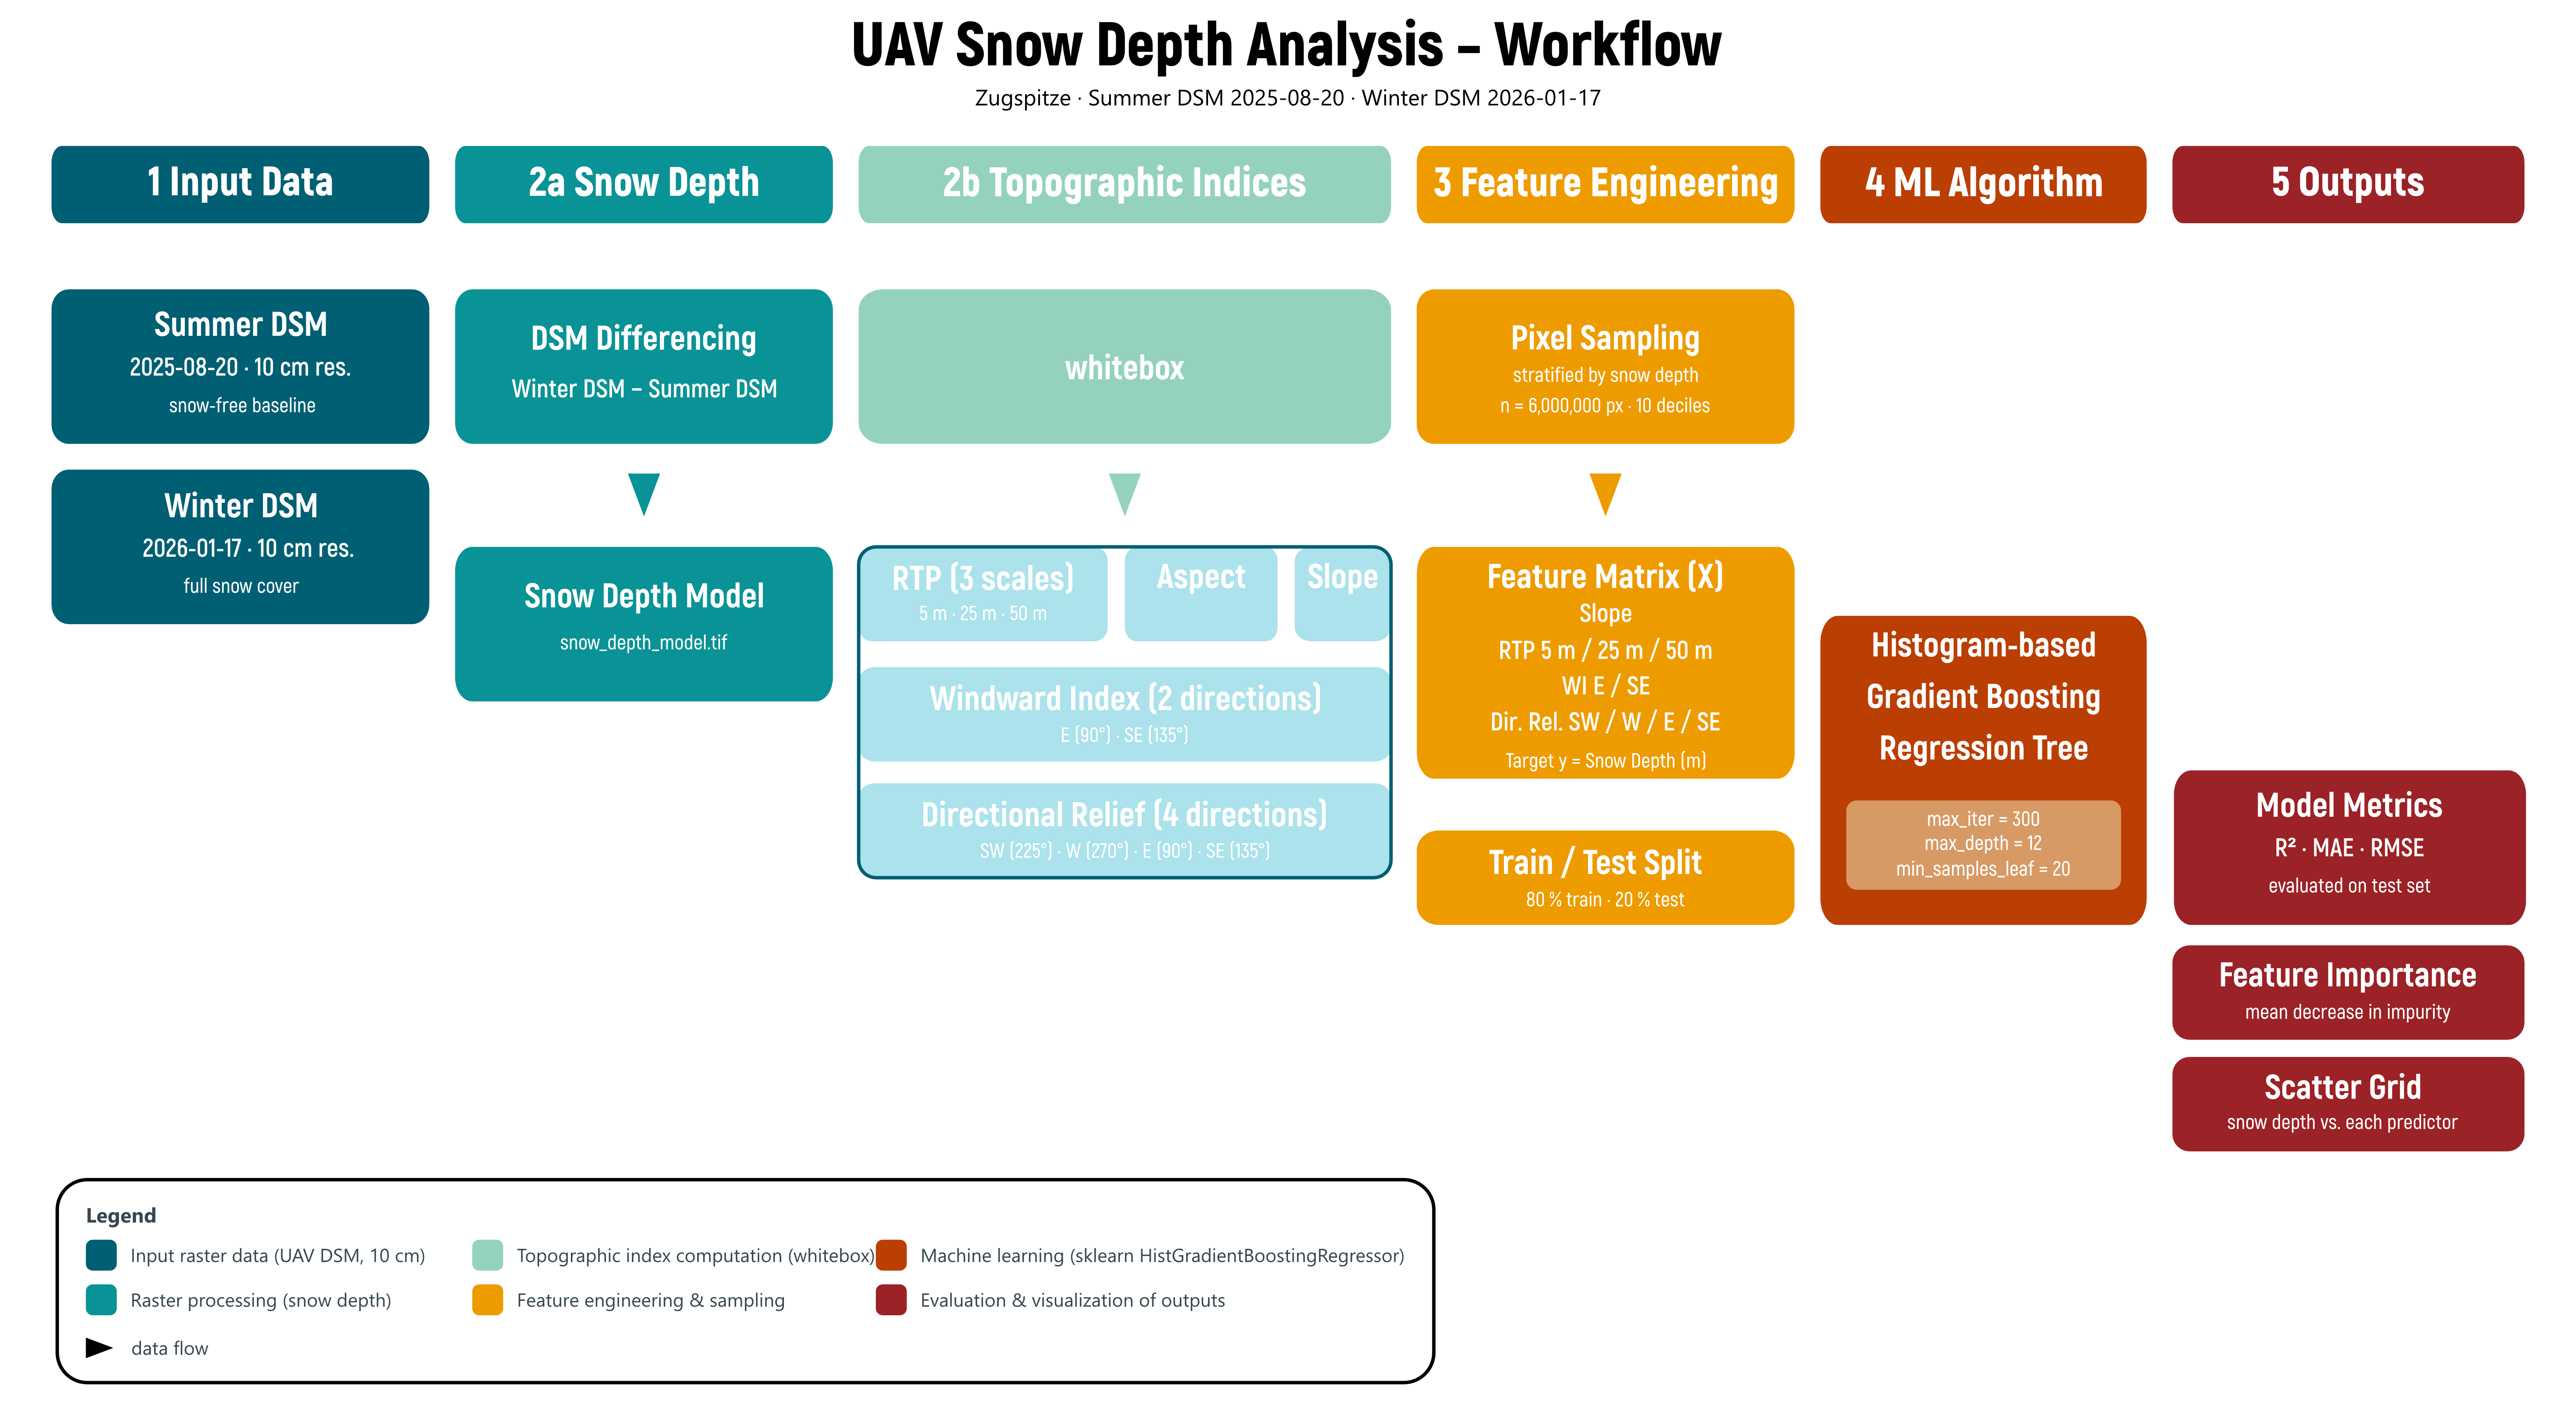
\includegraphics[width=0.8\columnwidth]{Figures/workflow_diagram.png}
		\caption{A flowchart visualising the workflow.}
	\end{center}
\end{figure}
\section*{\titleA{RESULTS}}

\vspace{1cm}
\noindent
\begin{minipage}[t]{0.48\linewidth}
  \centering
  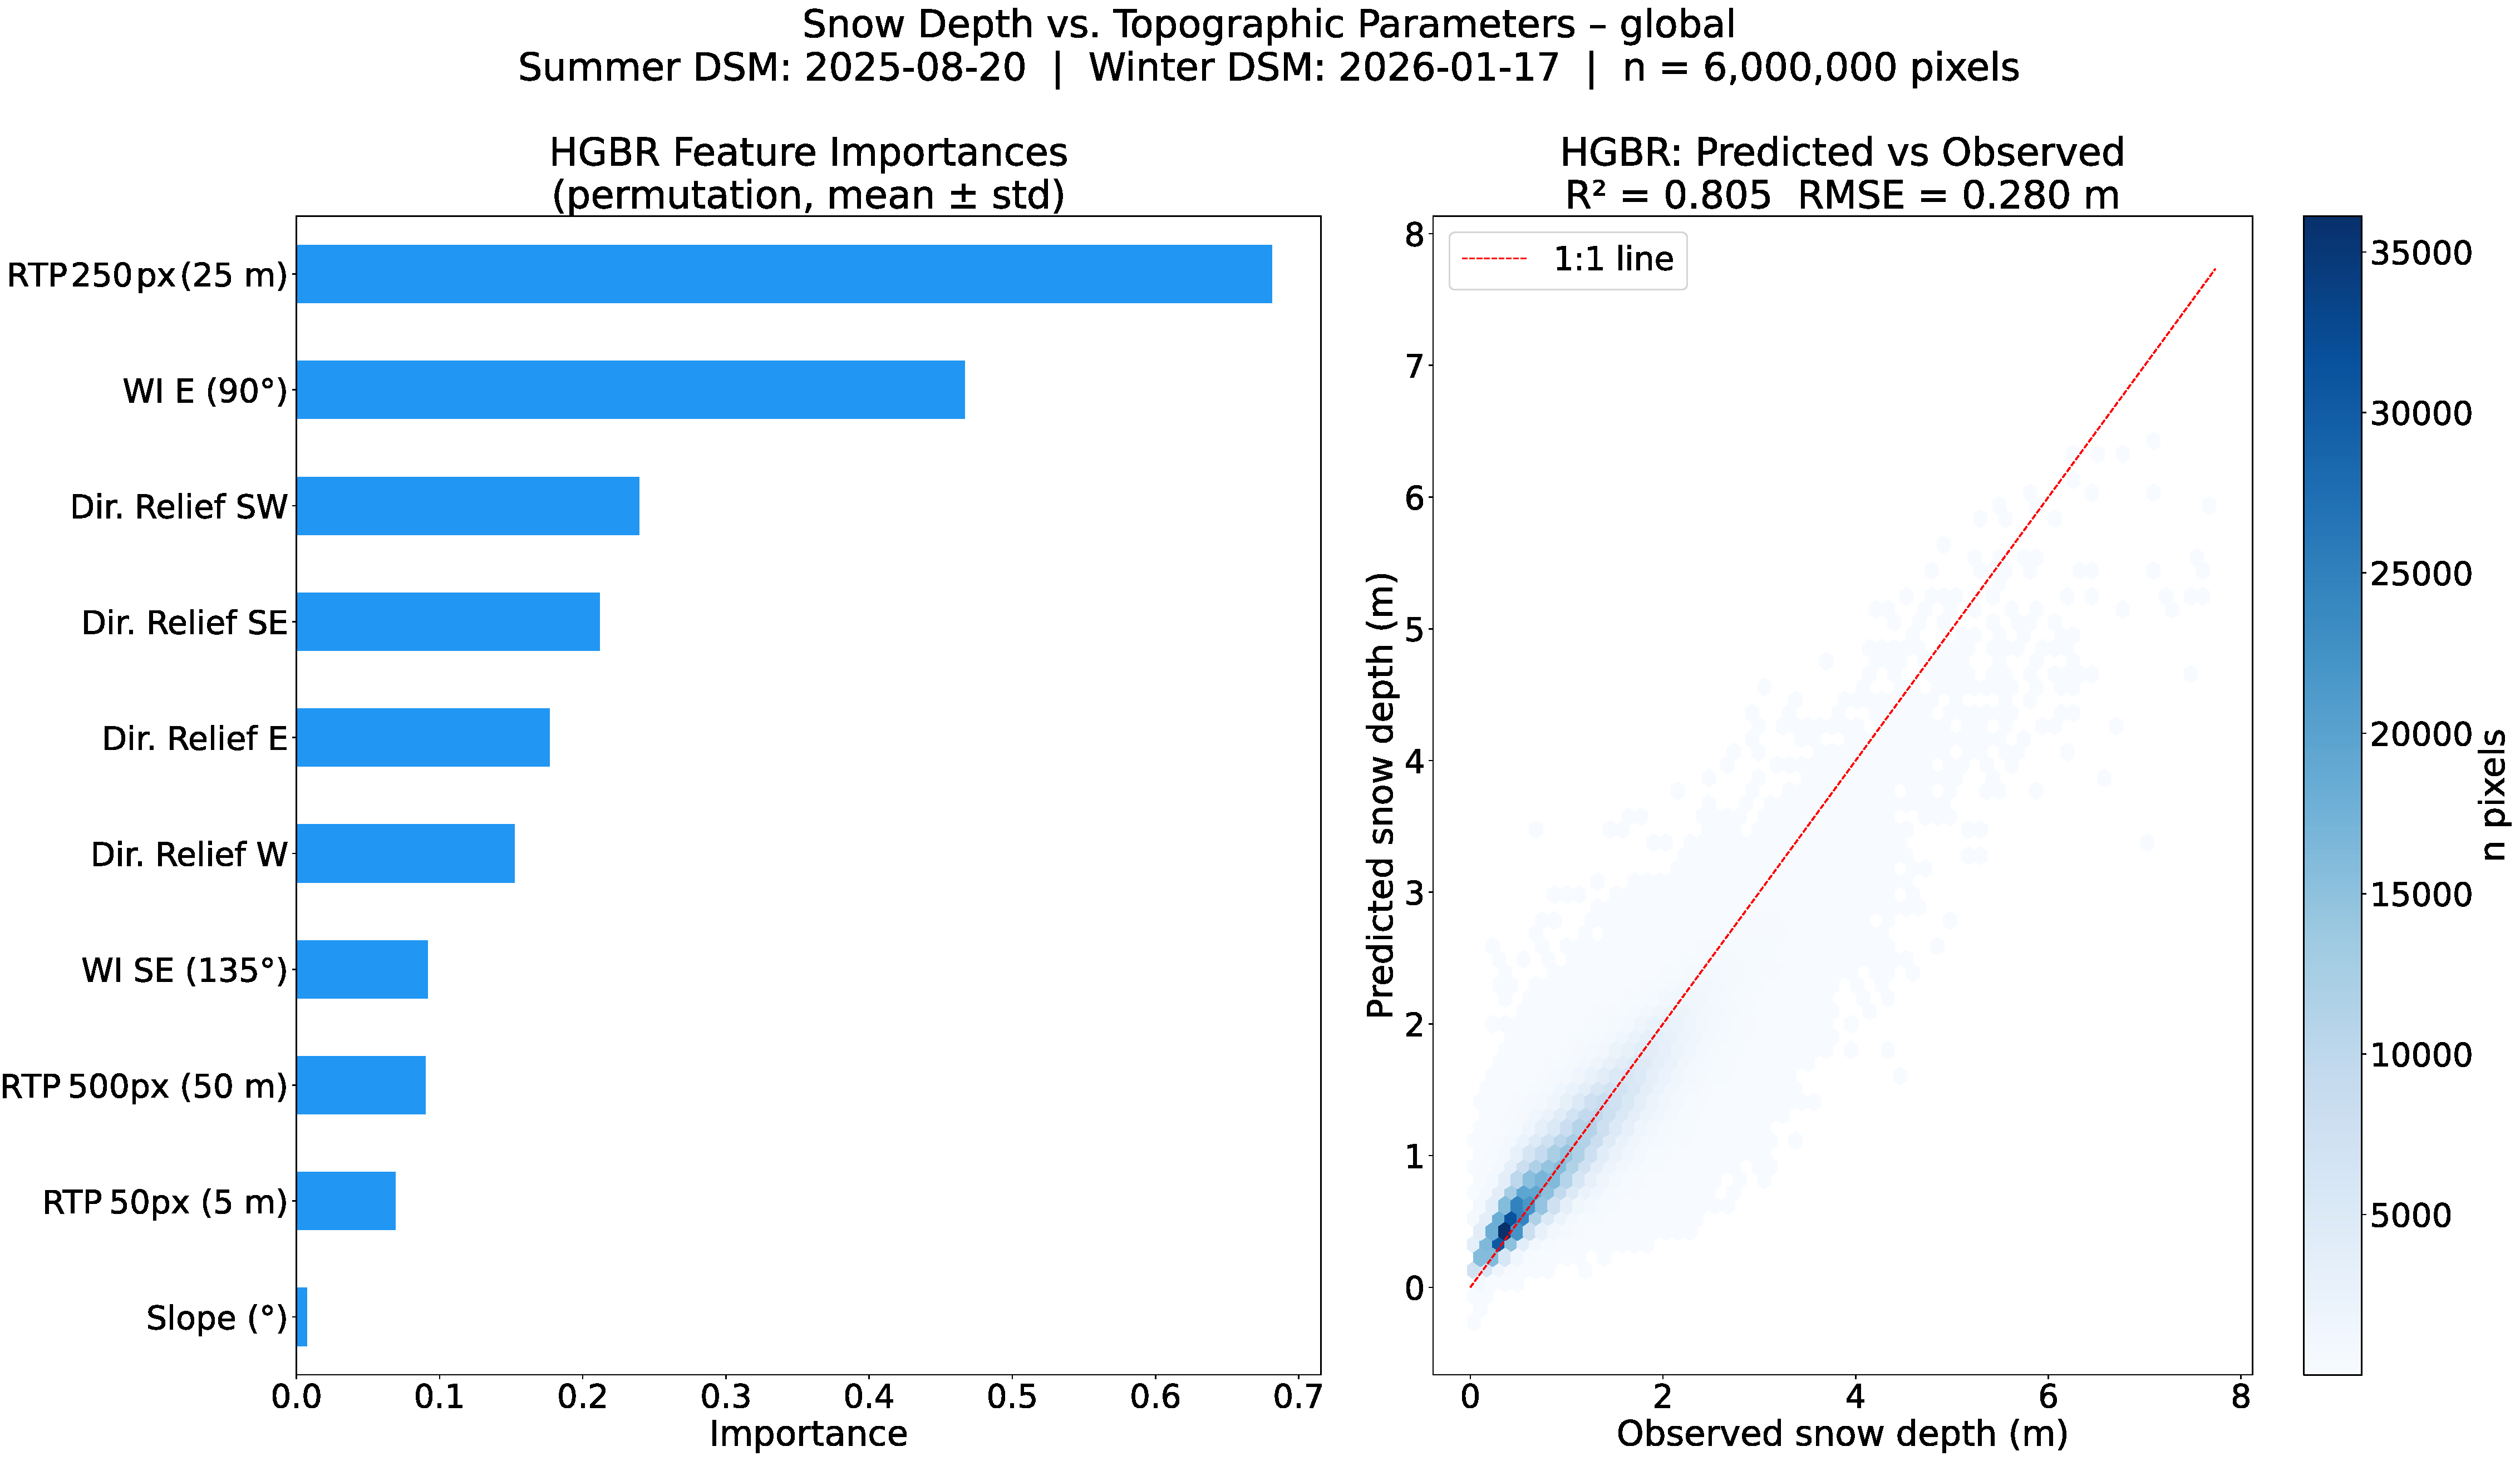
\includegraphics[width=\linewidth, height=0.26\textheight, keepaspectratio]{Figures/analysis_hbbr_new/global_analysis.pdf}
\end{minipage}
\hfill
\begin{minipage}[t]{0.48\linewidth}
  \centering
  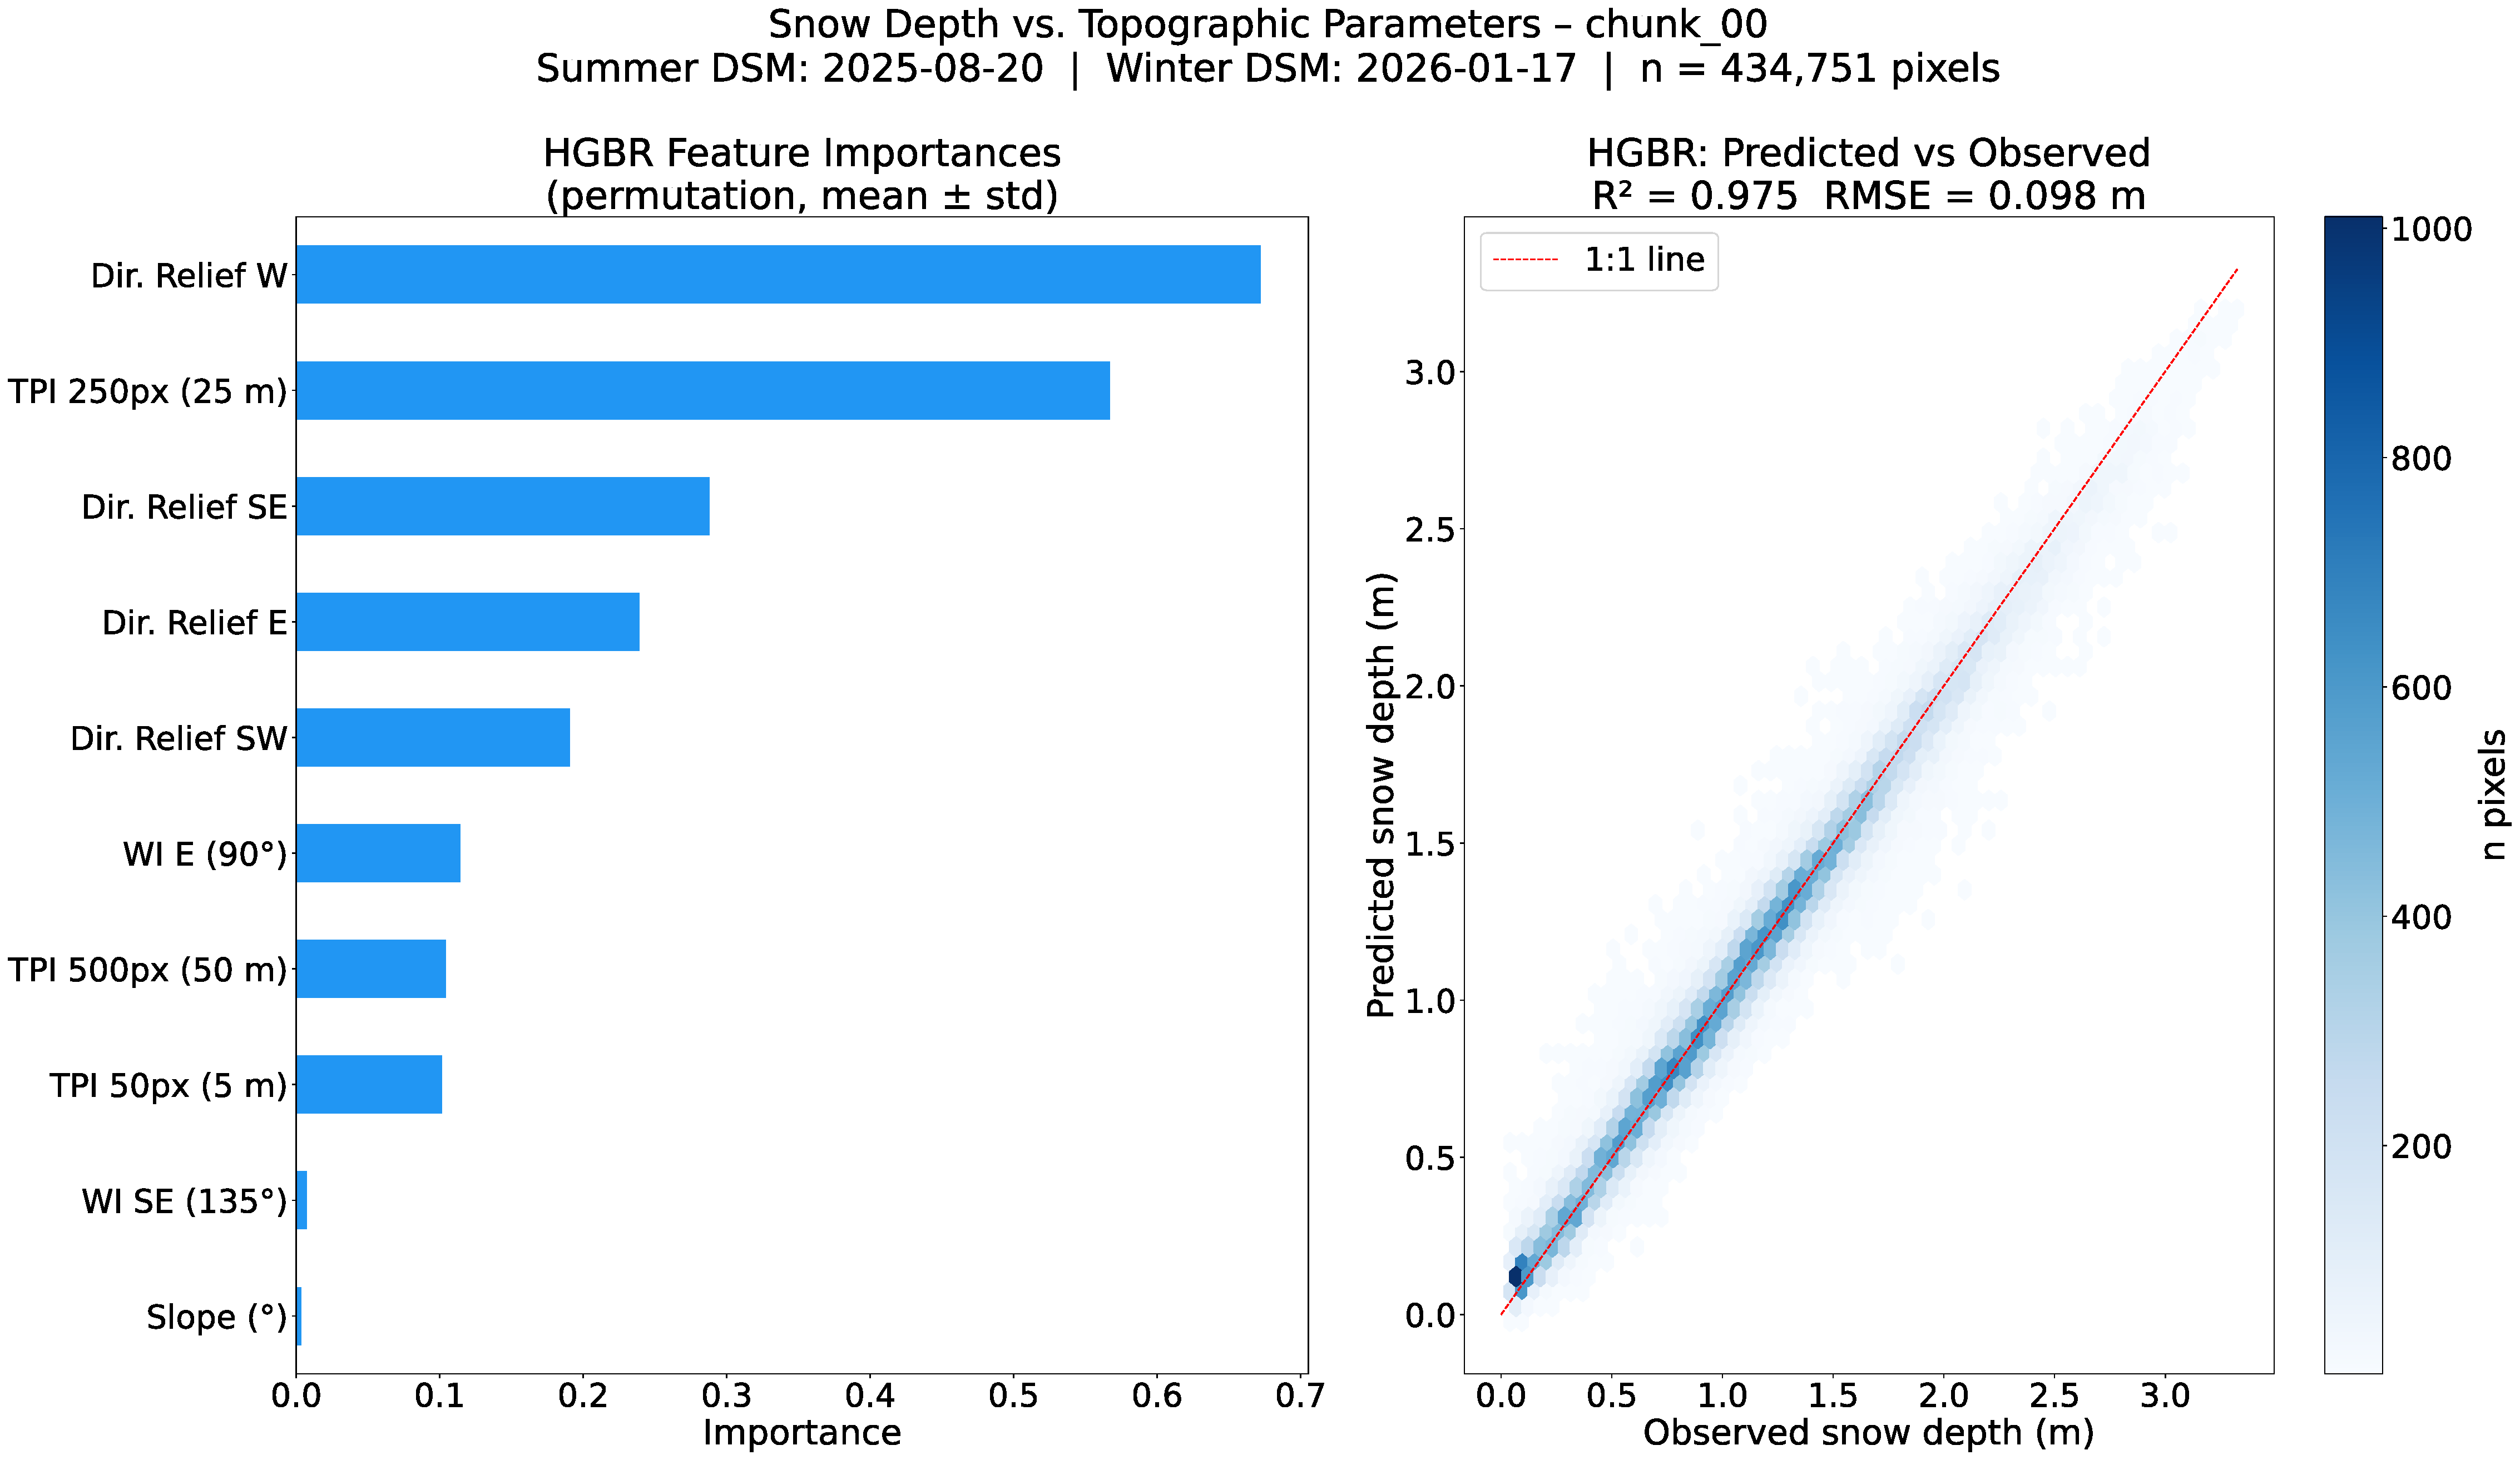
\includegraphics[width=\linewidth, height=0.26\textheight, keepaspectratio]{Figures/analysis_hbbr_new/chunks/chunk_00/chunk_00_analysis.pdf}
\end{minipage}
\captionof{figure}{Feature importances and predicted vs.\ observed snow depth:
global model (left) and Chunk\,00 as a representative subset (right).
TPI\,250\,px dominates globally; local models show varying feature hierarchies.}

\section*{\titleA{CONCLUSIONS}}

\noindent
The TPI at 25\,m scale is the dominant predictor ($R^2\!=\!0.805$, $\mathrm{RMSE}\!=\!0.280\,\mathrm{m}$
globally). Eastern wind exposure (windward index~E) is the most relevant wind factor;
all directional reliefs contribute. Chunk-wise modelling substantially improves accuracy
($R^2\!=\!0.969$, $\mathrm{RMSE}\!=\!0.114\,\mathrm{m}$), confirming spatial heterogeneity
in topography--snow relationships.

\input{Sections/References}
\end{multicols}
\end{document}